
% Copyright 2006, Tony R. Kuphaldt, released under the Creative Commons Attribution License (v 1.0)
% This means you may do almost anything with this work of mine, so long as you give me proper credit

%(BEGIN_FRONTMATTER)

\centerline{\bf Metric prefixes and conversion constants}

\begin{itemize}
\item{}{\bf Metric prefixes}
\item{}Yotta = 10$^{24}$ Symbol: Y
\item{}Zeta = 10$^{21}$ Symbol: Z
\item{}Exa = 10$^{18}$ Symbol: E
\item{}Peta = 10$^{15}$ Symbol: P
\item{}Tera = 10$^{12}$ Symbol: T
\item{}Giga = 10$^{9}$ Symbol: G
\item{}Mega = 10$^{6}$ Symbol: M
\item{}Kilo = 10$^{3}$ Symbol: k
\item{}Hecto = 10$^{2}$ Symbol: h
\item{}Deca = 10$^{1}$ Symbol: da
\item{}Deci = 10$^{-1}$ Symbol: d
\item{}Centi = 10$^{-2}$ Symbol: c
\item{}Milli = 10$^{-3}$ Symbol: m
\item{}Micro = 10$^{-6}$ Symbol: $\mu$
\item{}Nano = 10$^{-9}$ Symbol: n
\item{}Pico = 10$^{-12}$ Symbol: p
\item{}Femto = 10$^{-15}$ Symbol: f
\item{}Atto = 10$^{-18}$ Symbol: a
\item{}Zepto = 10$^{-21}$ Symbol: z
\item{}Yocto = 10$^{-24}$ Symbol: y
\end{itemize}

$$\includegraphics[width=15.5cm]{conversion_constantsx01.eps}$$

\goodbreak 
\begin{itemize}
\item{}{\bf Conversion formulae for temperature}
\item{}$^{o}$F = ($^{o}$C)(9/5) + 32
\item{}$^{o}$C = ($^{o}$F - 32)(5/9)
\item{}$^{o}$R = $^{o}$F + 459.67
\item{}K = $^{o}$C + 273.15
\end{itemize}
\bigskip 

%%%%%%%%%%%%%%%%%%%% 

\goodbreak 
{\bf Conversion equivalencies for distance}

\vskip 5pt {\narrower \noindent \baselineskip5pt
1 inch (in) = 2.540000 centimeter (cm)
\par} \vskip 5pt
{\narrower \noindent \baselineskip5pt
1 foot (ft) = 12 inches (in)
\par} \vskip 5pt
{\narrower \noindent \baselineskip5pt
1 yard (yd) = 3 feet (ft)
\par} \vskip 5pt
{\narrower \noindent \baselineskip5pt
1 mile (mi) = 5280 feet (ft)
\par} \vskip 10pt
\bigskip 
 
%%%%%%%%%%%%%%%%%%%% 

\goodbreak 
{\bf Conversion equivalencies for volume}

\vskip 5pt {\narrower \noindent \baselineskip5pt
1 gallon (gal) = 231.0 cubic inches (in$^{3}$) = 4 quarts (qt) = 8 pints (pt) = 128 fluid ounces (fl. oz.) = 3.7854 liters (l)
\par} \vskip 5pt
\vskip 5pt {\narrower \noindent \baselineskip5pt
1 milliliter (ml) = 1 cubic centimeter (cm$^{3}$)
\par} \vskip 10pt
\bigskip 
 
%%%%%%%%%%%%%%%%%%%% 

\goodbreak 
{\bf Conversion equivalencies for velocity}

\vskip 5pt {\narrower \noindent \baselineskip5pt
1 mile per hour (mi/h) = 88 feet per minute (ft/m) = 1.46667 feet per second (ft/s) = 1.60934 kilometer per hour (km/h) = 0.44704 meter per second (m/s) = 0.868976 knot (knot -- international)
\par} \vskip 10pt
\bigskip 
 
%%%%%%%%%%%%%%%%%%%% 

\goodbreak 
{\bf Conversion equivalencies for mass}

\vskip 5pt {\narrower \noindent \baselineskip5pt
1 pound (lbm) = 0.45359 kilogram (kg) = 0.031081 slugs
\par} \vskip 10pt
\bigskip 
 
%%%%%%%%%%%%%%%%%%%% 

\goodbreak 
{\bf Conversion equivalencies for force}

\vskip 5pt {\narrower \noindent \baselineskip5pt
1 pound-force (lbf) = 4.44822 newton (N)
\par} \vskip 10pt
\bigskip 
 
%%%%%%%%%%%%%%%%%%%% 

\goodbreak 
{\bf Conversion equivalencies for area}

\vskip 5pt {\narrower \noindent \baselineskip5pt
1 acre = 43560 square feet (ft$^{2}$) = 4840 square yards (yd$^{2}$) = 4046.86 square meters (m$^{2}$)
\par} \vskip 10pt
\bigskip 
 
%%%%%%%%%%%%%%%%%%%% 

\goodbreak 
{\bf Conversion equivalencies for common pressure units (either all gauge or all absolute)}

\vskip 5pt {\narrower \noindent \baselineskip5pt
1 pound per square inch (PSI) = 2.03602 inches of mercury (in. Hg) = 27.6799 inches of water (in. W.C.) = 6.894757 kilo-pascals (kPa) = 0.06894757 bar
\par} 
\medskip 
 
{\narrower \noindent \baselineskip5pt
1 bar = 100 kilo-pascals (kPa) = 14.504 pounds per square inch (PSI) 
\par} \vskip 10pt
\bigskip 

%%%%%%%%%%%%%%%%%%%% 

\goodbreak 
{\bf Conversion equivalencies for absolute pressure units (only)}

\vskip 5pt {\narrower \noindent \baselineskip5pt
1 atmosphere (Atm) = 14.7 pounds per square inch absolute (PSIA) = 101.325 kilo-pascals absolute (kPaA) = 1.01325 bar (bar) = 760 millimeters of mercury absolute (mmHgA) = 760 torr (torr)
\par} \vskip 10pt
\bigskip 

%%%%%%%%%%%%%%%%%%%% 

\goodbreak 
{\bf Conversion equivalencies for energy or work}

\vskip 5pt {\narrower \noindent \baselineskip5pt
1 british thermal unit (Btu -- ``International Table'') = 251.996 calories (cal -- ``International Table'') = 1055.06 joules (J) = 1055.06 watt-seconds (W-s) = 0.293071 watt-hour (W-hr) = 1.05506 x 10$^{10}$ ergs (erg) = 778.169 foot-pound-force (ft-lbf) 
\par} \vskip 10pt
\bigskip 
 
%%%%%%%%%%%%%%%%%%%% 

\goodbreak 
{\bf Conversion equivalencies for power}

\vskip 5pt {\narrower \noindent \baselineskip5pt
1 horsepower (hp -- 550 ft-lbf/s) = 745.7 watts (W) = 2544.43 british thermal units per hour (Btu/hr) = 0.0760181 boiler horsepower (hp -- boiler)
\par} \vskip 10pt
\bigskip 
 
%%%%%%%%%%%%%%%%%%%% 

\goodbreak 
{\bf Acceleration of gravity (free fall), Earth standard}

\vskip 5pt {\narrower \noindent \baselineskip5pt
9.806650 meters per second per second (m/s$^{2}$) = 32.1740 feet per second per second (ft/s$^{2}$)
\par} \vskip 10pt
\bigskip 
 
%%%%%%%%%%%%%%%%%%%% 

\goodbreak 
{\bf Physical constants}

\vskip 5pt {\narrower \noindent \baselineskip5pt
Speed of light in a vacuum ($c$) = 2.9979 $\times$ $10^8$ meters per second (m/s) = 186,281 miles per second (mi/s)
\par} \vskip 5pt
\vskip 5pt {\narrower \noindent \baselineskip5pt
Avogadro's number ($N_A$) = 6.022 $\times$ $10^{23}$ per mole (mol$^{-1}$)
\par} \vskip 5pt
\vskip 5pt {\narrower \noindent \baselineskip5pt
Electronic charge ($e$) = 1.602 $\times$ $10^{-19}$ Coulomb (C)
\par} \vskip 5pt
\vskip 5pt {\narrower \noindent \baselineskip5pt
Boltzmann's constant ($k$) = 1.38 $\times$ $10^{-23}$ Joules per Kelvin (J/K)
\par} \vskip 5pt
\vskip 5pt {\narrower \noindent \baselineskip5pt
Stefan-Boltzmann constant ($\sigma$) = 5.67 $\times$ $10^{-8}$ Watts per square meter-Kelvin$^{4}$ (W/m$^{2} \cdot$K$^{4}$)
\par} \vskip 5pt
\vskip 5pt {\narrower \noindent \baselineskip5pt
Molar gas constant ($R$) = 8.314 Joules per mole-Kelvin (J/mol-K)
\par} \vskip 10pt
\bigskip 
 
%%%%%%%%%%%%%%%%%%%% 

\goodbreak 
{\bf Properties of Water}

\vskip 5pt {\narrower \noindent \baselineskip5pt
Freezing point at sea level = 32$^{o}$F = 0$^{o}$C
\par} \vskip 5pt
\vskip 5pt {\narrower \noindent \baselineskip5pt
Boiling point at sea level = 212$^{o}$F = 100$^{o}$C
\par} \vskip 5pt
\vskip 5pt {\narrower \noindent \baselineskip5pt
Density of water at 4$^{o}$C = 1000 kg/m$^{3}$ = 1 g/cm$^{3}$ = 1 kg/liter = 62.428 lb/ft$^{3}$ = 1.94 slugs/ft$^{3}$
\par} \vskip 5pt
\vskip 5pt {\narrower \noindent \baselineskip5pt
Specific heat of water at 14$^{o}$C = 1.00002 calories/g$\cdot$$^{o}$C = 1 BTU/lb$\cdot$$^{o}$F = 4.1869 Joules/g$\cdot$$^{o}$C
\par} \vskip 5pt
\vskip 5pt {\narrower \noindent \baselineskip5pt
Specific heat of ice $\approx$ 0.5 calories/g$\cdot$$^{o}$C
\par} \vskip 5pt
\vskip 5pt {\narrower \noindent \baselineskip5pt
Specific heat of steam $\approx$ 0.48 calories/g$\cdot$$^{o}$C
\par} \vskip 5pt
\vskip 5pt {\narrower \noindent \baselineskip5pt
Absolute viscosity of water at 20$^{o}$C = 1.0019 centipoise (cp) = 0.0010019 Pascal-seconds (Pa$\cdot$s)
\par} \vskip 5pt
\vskip 5pt {\narrower \noindent \baselineskip5pt
Surface tension of water (in contact with air) at 18$^{o}$C = 73.05 dynes/cm
\par} \vskip 5pt
\vskip 5pt {\narrower \noindent \baselineskip5pt
pH of pure water at 25$^{o}$ C = 7.0 ({\it pH scale = 0 to 14})
\par} \vskip 10pt
\bigskip 
 
%%%%%%%%%%%%%%%%%%%% 

\goodbreak 
{\bf Properties of Dry Air at sea level}

\vskip 5pt {\narrower \noindent \baselineskip5pt
Density of dry air at 20$^{o}$C and 760 torr = 1.204 mg/cm$^{3}$ = 1.204 kg/m$^{3}$ = 0.075 lb/ft$^{3}$ = 0.00235 slugs/ft$^{3}$
\par} \vskip 5pt
\vskip 5pt {\narrower \noindent \baselineskip5pt
Absolute viscosity of dry air at 20$^{o}$C and 760 torr = 0.018 centipoise (cp) = 1.8 $\times$ $10^{-5}$ Pascal-seconds (Pa$\cdot$s)
\par} \vskip 5pt
\bigskip 
 

% Note: most of these constants and conversion factors came from the 64th edition of the CRC Handbook of Chemistry and Physics.

\vfil

\underbar{file {\tt conversion\_constants}}
\eject
%(END_FRONTMATTER)

